\documentclass[a4paper, 11pt, article]{report}
\usepackage[font={small,it}]{caption}
\usepackage[pagestyles]{titlesec}
\usepackage[utf8]{inputenc}
\usepackage{graphicx}
\usepackage{listings}
\usepackage{float}
\usepackage{todonotes}

\begin{document}

\titleformat{\chapter}{\bf\huge}{\thechapter}{20pt}{\huge}

%%%%%%%%%%%%%%%%%%%%%%%%%%%%%%%%%%%%%%%%%%%%%%%%%%%%%%%%%%%%%%%%%%%%%%%%%%%%%%%%%%%%%%%%%%%%%%%%%%%%%%%
   
\begin{titlepage}
	\newcommand{\HRule}{\rule{\linewidth}{0.5mm}}
	\center
	
    \textsc{\LARGE Cranfield University}\\[0.8cm]
    
\includegraphics[width=2cm]{images/cranfield}\\[0.8cm]
    \textsc{\Large MSc in Computational and Software Techniques in Engineering 2016/2017}\\[0.8cm]
    \textsc{\large Software Engineering in Technical Computing}\\
    \textsc{\large School of Aerospace, Transport and Manufacturing}\\[1.1cm]
       
    \HRule \\[0.4cm]
    {\huge \bfseries Applications in Practical  \\[0.5cm]
    	High-End Computing}\\[0.3cm]
    \LARGE\HRule \\[1.5cm]
       
    \begin{minipage}{1.1\textwidth}
    	\begin{flushleft} \large
        	{Authors}\\
            Andreas \textbf{Schmidhofer} \\
            Gergő \textbf{Szűcs} \\
            Paweł \textbf{Żybura} \\ 
            Piotr \textbf{Kaźmierczak} \\
            Xin \textbf{Lu}
        \end{flushleft}
    \end{minipage}
	\\[0.9cm] 
    \begin{minipage}{0.9\textwidth}
    	\begin{flushright} \large
        	{Supervisors}
            \\ Dr Dominique \textbf{Fleischmann}
            \\ Dr  Irene \textbf{Moulitsas}
        \end{flushright}
    \end{minipage}\\[1cm]
       
    \vfill
    {\large \today}
    \clearpage
\end{titlepage}

%%%%%%%%%%%%%%%%%%%%%%%%%%%%%%%%%%%%%%%%%%%%%%%%%%%%%%%%%%%%%%%%%%%%%%%%%%%%%%%%%%%%%%%%%%%%%%%%%%%%%%%

\tableofcontents
\newpage

\chapter{Introduction}

In this paper we will discuss the project we had to complete for the Applications in Practical High-End Computing, as well as giving \textbf{insight to the team}, the way we worked throughout the weeks, the \textbf{approaches we took} and the \textbf{results we have achieved}.

The kick-off of the project was five days of introduction of the software, where we had the chance to familiarise ourselves with the concept of the application, its purpose and the source code itself. We were also given many hints and ideas about the possible features and improvements. However, it was emphasised that we were expected to \textbf{think out of the box}, try to \textbf{create something extraordinary}, while still focusing on the feasibility of software for our future customers.

\section{Our vision of the project}

The major idea we had was to \textbf{explore as many aspects of improvement as possible}. First of all we wanted to apply our already existing software engineering knowledge and everything we had learnt during the Requirements Analysis and System Design course and make sure the source code employs the \textbf{best practices for both efficiency and readability}.

During the first days of the project we realised that it is a bit cumbersome to set-up the environment and have the code running. Due to that we wanted to make sure the whole package is as user friendly as possible, by \textbf{removing} most of the \textbf{third party dependencies}, by including them into the deployment and providing a \textbf{standalone installer} for the customers.

Our market analysis had shown that the potential users have troubles using the software. Most of their concerns were about the layout and handling of the graphical interface and the necessity of having three different applications. This put our focus on \textbf{merging two} of the existing \textbf{applications} together and providing convenient access between the remaining two, while also adding  quality of life features to the user interface.

Another drawback of the software is the strict requirement of a CUDA enabled graphical card, which may not be available for many of our customers. Since this is a must because of the complexity of the computations in FlexIT, our idea was to provide \textbf{cloud access to the software} for these customers. In this case, the application would run on a Windows server with a feasible GPU, removing the dependency from the user side.

Creating the meshes in SurfIT was also more complicated than most of the customers would like, and there are many existing software out there for this task, one of the most famous is CAD. We explored the possibilities of \textbf{importing} the different type of \textbf{models from CAD} into our application, allowing the user to create meshes faster or even use existing ones.

Apart from these ambitious ideas, we also aimed to work on the existing source code, \textbf{implement missing features}, \textbf{fix existing bugs} and in general, \textbf{make the program faster and the user-experience smoother}.


\section{The team}

Our team was based on diversity in both nationalities and expertise. We knew that the project is not only about making the best software, but to understand the big picture, \textbf{create an achievable common goal and work towards that as a team}. 

Mixing \textbf{multiple disciplines} in the group helped us a lot to come up with a wide variety of ideas, while the \textbf{cultural diversity} allowed us to learn about the mindset and behaviour of people from different nationalities. As we are in a software engineering course, the majority of the expertise came from this field, while also having decent amount of mechatronical and  mechanical engineering, as well as mathematics knowledge. Due to the recent Management for Technology course, we were familiar with many aspects of managements, including marketing, which was a big part of the project. \\[0.3cm]

\newpage 

\begin{minipage}{0.3\textwidth}\raggedleft
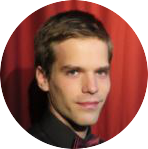
\includegraphics[width=2.5cm]{images/andy}
\end{minipage}
\hfill
\begin{minipage}{0.7\textwidth}\center
Andreas \textbf{Schmidhofer} \\   
Austria \\
Computer scientist
\end{minipage} \\[1.5cm]

\begin{minipage}{0.4\textwidth}\center
Gergő \textbf{Szűcs} \\   
Hungary \\
Software engineer
\end{minipage}%
\hfill%
\begin{minipage}{0.4\textwidth}\raggedright
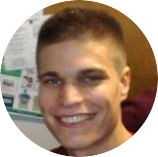
\includegraphics[width=2.5cm]{images/gergo}
\end{minipage} \\[1.5cm]

\begin{minipage}{0.3\textwidth}\raggedleft

\includegraphics[width=2.5cm]{images/pawel}
\end{minipage}
\hfill
\begin{minipage}{0.7\textwidth}\center
Paweł \textbf{Żybura} \\   
Poland \\
Mechatronical engineer
\end{minipage} \\[1.5cm]

\begin{minipage}{0.4\textwidth}\center
Piotr \textbf{Kaźmierczak} \\  
Poland \\
Mechanical engineer
\end{minipage}%
\hfill%
\begin{minipage}{0.4\textwidth}\raggedright

\includegraphics[width=2.5cm]{images/piotr}
\end{minipage} \\[1.5cm]

\begin{minipage}{0.3\textwidth}\raggedleft

\includegraphics[width=2.5cm]{images/xin}
\end{minipage}
\hfill
\begin{minipage}{0.7\textwidth}\center
Xin \textbf{Lu} \\   
China \\
Mathematician
\end{minipage}

%%%%%%%%%%%%%%%%%%%%%%%%%%%%%%%%%%%%%%%%%%%%%%%%%%%%%%%%%%%%%%%%%%%%%%%%%%%%%%%%%%%%%%%%%%%%%%%%%%%%%%%

\chapter{Work organization}

In general, we felt that our groups was working quite effectively, keeping in mind that we had assignments and thesis work as well during the group project's period. Every team member was proactive and perceptive during our meetings, while we were also be able to work on our own when it was required.
   
\section{Meetings}

During the project all group members had stayed on campus, allowing us to \textbf{meet in person regularly} and sometimes on exceptional occasions. We have held our regular meetings twice a week, usually on Monday and Thursday. On these occasions, we have told each other about the progress we had made, since the previous meeting and discussed the tasks for the next period of time, while also helping each other with the problems and questions, which we could not solve alone.

We always \textbf{rotated the role of the meeting leader} in our group, to make sure everyone can get familiar with the aspect of it, while also making sure there is always a person to control the flow of these gatherings. The meetings usually took around 30-40 minutes, including the time while we added our notes and tasks to Trello, to make sure we have some footprint of the meeting.

Every now and then one of the group members faced critical problems, which would have caused delay in our progression, hence they needed to call an \textbf{emergency meetings}. These meetings were not always for the whole group, but for the people who could help the person in need. Thankfully, we did not have too many of these critical situations, and every group member was glad to help each other.
   
\section{External tools}

As we mentioned before, we had used quite a few tools to manage our project. 

\textbf{Trello} was our project management tools, which made handling the tasks and deadlines effortless. We set up different type of lists, where we initially added all our ideas. During our work, we always added the new ideas and bugs to the list, to make sure everyone know about their existence. These tasks then were assigned to people and given a deadline during our meetings. This allowed us to easily follow what each person was working on at the given time.

To make sure we are able to follow the dynamic nature of the project and synchronize our work efficiently, we put our source code into a private \textbf{GitHub repository}. This let us to share our changes in the source code with each other easily, and keep track of the changes we made. We could also try out \textbf{experimental features} on branches and merging the promising ones back to the trunk later. Apart from these, it provided us with some interesting feedback on our work, for example the usual days and hours of commits, the distribution of the programming languages in the code base, etc.

\section{Project timeline}

While our original plan did not exactly come through (due to unexpected issues, new ideas and delays), we have managed to do most of the initial ideas.

\begin{figure}[H]
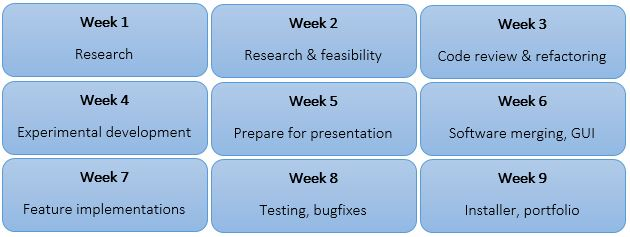
\includegraphics[width=12.8cm]{images/weeklyplan}
\caption{High level initial weekly plan}
\centering
\end{figure}

We will discuss all of the work we carried out in different sections later in this paper.

\section{Individual contribution}

As this was a group project, most of our achievements would not had been possible individually. \textbf{What we have done is the great effort of the whole team}, however here are the parts that each individual mostly worked on. Keep in mind, that we have helped each other in most of the tasks, to allow greater efficiency and faster problem solving. \\

\noindent Andreas \textbf{Schmidhofer} 
\begin{itemize}
	\item Requirement analysis
	\item Design
	\item Researching cloud computing possibilities
	\item Preparing the presentation
	\item Testing on the Amazon cloud
	\item Creating and editing video for the presentation
	\item Preparing the portfolio
\end{itemize} 

\noindent \\ Gergő \textbf{Szűcs}
\begin{itemize}
	\item Requirement analysis
	\item Design
	\item Code review
	\item Code refactoring
	\item Removing third party dependencies
	\item Fixing packaging issues
	\item DesignIT and FlexIT interfacing
	\item Preparing the presentation
	\item Detecting and fixing memory leaks
	\item Testing 
	\item Graceful handling of errors and exceptions
	\item Bugfixing
	\item Installer creation
	\item Performance measurements
	\item Preparing the portfolio
\end{itemize}

\noindent \\ Paweł \textbf{Żybura} 
\begin{itemize}
	\item Requirement analysis
	\item Design
	\item Code review
	\item Merging SurfIT and MoveIT into DesignIT
	\item Command line feature
	\item Preparing the presentation
	\item Merging views to one class
	\item GUI redesign
	\item Undo-redo functionality
	\item Testing 
	\item Bugfixing
	\item Preparing the portfolio
\end{itemize}

\noindent \\ Piotr \textbf{Kaźmierczak} 
\begin{itemize}
	\item Market analysis
	\item Test plan
	\item CAD research
	\item Preparing the presentation
	\item Preparing the portfolio
\end{itemize}

\noindent \\ Xin \textbf{Lu}
\begin{itemize}
	\item Market analysis
	\item Test plan
	\item Mathematics research
	\item Preparing the presentation
	\item Implementing new liner equation solver
	\item Preparing the portfolio
\end{itemize}

%%%%%%%%%%%%%%%%%%%%%%%%%%%%%%%%%%%%%%%%%%%%%%%%%%%%%%%%%%%%%%%%%%%%%%%%%%%%%%%%%%%%%%%%%%%%%%%%%%%%%%%

\chapter{Research}

\section{Market analysis}

\section{Mathematics and algorithms}

\section{Cloud computing}

\section{Importing CAD models}
   
There are many CAD programs but the most popular program in the world is Autocad. It allows you to design two- and three-dimensional coordinate systems and save drawings to a DWG file.

DWG files are a standard for CAD applications. Unfortunately due to the fact that it is a closed binary format reserved by Autodesk, Autocad is required for DWG files. Fortunately, you can also use breaking monopoly programming libraries created by other companies such as Open Design Alliance (formerly OpenDWG).

Autodesk has released a number of specialized overlays such as AutoCAD Electrical, AutoCAD Mechanical, Mechanical Desktop, Architectural Desktop, and Civil Design that require AutoCAD to be the "engine" that manages their work.

In addition, it has provided many programming interfaces for writing custom extensions for Autocad.

\subsection{AutoLisp}

It is a variation of the Lisp script language adapted for Autocad to automate repetitive operations and increase productivity. For example, calculating the total length of all lines in a drawing - imagine how long it would take to count that.

The great advantage of Autolisp is that you do not need much programming knowledge to use it. Even a beginner Autocad user can create a simple algorithm that will save him hours or days of work.

Another advantage is its portability, as Autodesk did not develop it by moving its attention to another VisualLisp language, it was implemented in the same form in most "clones", so the application written in Autolisp should equally work in Autocad as in Intellicad.

AutoLisp is a scripting language which on the one hand can be considered as an advantage (no special programming environment is needed) and on the other hand, it is a big disadvantage, because the scripting language is interpreted during execution, so extensions in it are characterized by slow action.

The entire application code written in AutoLisp is visible to anyone who opens code files which is a big minus for commercial programs, no one wants his hard work to be used illegally by others.

In summary, AutoLisp is rather an enhancement for engineers wishing to accelerate the tedious task of writing applications for sale.

\subsection{VisualLisp}

VisualLisp was designed as an extension of AutoLisp functionality. Its capabilities are much more powerful than AutoLisp, it has access to the Autocad object model. In addition, the development environment has been implemented in Autocad so developers no longer need to use external editors (as opposed to AutoLisp).

It was introduced in the Autocad version 14 as a paid add-on, then later added permanently. But since then, it has been abandoned by Autodesk, which has focused its efforts on more powerful programming interfaces.

VisualLisp as AutoLisp continues to reproduce most of its limitations and are therefore suitable for professional use.

\subsection{DCL}
   
With the help of AutoLisp and VisualLisp, one can not fail to mention the Dialog Control Language (DCL), which makes it easy to build dialog boxes with simple tags.

DCL has very limited capabilities, no language support is available from the Autocad command line.

\subsection{VBA}

Visual Basic for Application is derived from Microsoft Visual Basic and used in many different applications, including Autocad. In Autocad it obtains access to objects via the ActiveX interface.

ActiveX Automotion was introduced to Autocad at the same time as VisualLisp.

No further development of VisualLisp can be attributed to the fact that VBA had the advantage over it in the form of a built-in dialog box.

In 2007, Microsoft stopped supporting Autodesk in distributing this technology, encouraging developers to use the .Net API.

Autodesk has pushed out unauthorized Microsoft support to 2010, currently no longer has the development environment for VBA, and the language is no longer being developed.

\subsection{ADS}

Autocad Development System is a set of libraries written in C language. This interface allows you to create applications for Autocad in C and C++.

An external programming environment and programming expertise is needed to create an overlay using ADS.

Compared to previous technologies, the speed of C/C++ programming is increasing significantly, and the possibilities of application development are almost unlimited. You can not only insert parameterized blocks, but also "plug" into Autocad message loops or overwrite the default functionality of built-in functions.

The big plus of this technology was until recently that most of the "clones" implemented various variants, most of the functions overlapped - so when typing the overlay, it was very likely that without major problems (separate compilation with the appropriate CAD libraries) it will work on Autocad and Intellicad. Obviously, in the "clones" implementations of subsequent interfaces appear, but they have a long delay in relation to the Autodesk original.

The basic data structure in ADS is resbuf, which contains messages about the type of data contained in it, values written in union form, and pointer to the next resbuf element.
 
\subsection{ObjectARX}

Autocad Runtime eXtension is an API that is the next stage in extending Autocad functionality, which includes a set of libraries and C++ header files. All SDKs can be downloaded for free from Autodesk sites.

ObjectARX is the most powerful of all available interfaces, contains all the elements that are available in ADS and develops them with additional functionality.

The performance of this technology is the same as the performance of Autocad's own functions, and Autodesk's use of Autocad extensions such as Autodesk MAP and Architectural Desktop can also be attributed to Autodesk.

Of course, Autocad treading on the heels of the competition is trying to make portability portable. Clones based on the DWGDirect library of the Open Design Alliance have the ability to use the ObjectARX-DRX emulation API (eg Intellicad since version 7, previous versions only implemented ADS).

Some say that ObjectARX is the hardest interface for a programmer although I would bet that it is easier than ADS. However, to get started with it requires knowledge of programming in C ++ and an external development environment (eg Microsoft Visual Studio).

\subsection{DWG}
   
DWG - a proprietary binary file format created by AutoCAD.
This format was created by Autodesk to support AutoCAD software and derivative programs. Two- and three-dimensional models are written in this format. The owner of the format, Autodesk, distributes it and changes it once every few years with the release of the new version of AutoCAD.
DWG format with ASCII variant - DXF has become de facto standard format for CAD design.

The proprietary format DWG is currently the most used file format in CAD, becoming a standard, without other alternative extended, forcing many users to use this software in a dominant position on the part of the owner company Autodesk.
There exists the OpenDWG library, to access and manipulate data stored in DWG format, which is developed by reverse engineering by an association of manufacturers of CAD software with the intention of supporting their products. As OpenDWG's license does not allow the usage in free software projects, the FSF wants to create an alternative to OpenDWG.

\subsubsection{DWG Support in Freemium and Free Software}

As neither RealDWG nor DWGdirect are licensed on terms that are compatible with free software licenses like the GNU GPL, in 2008 the Free Software Foundation asserted the need for an open replacement for the DWG format. Therefore, the FSF placed the goal 'Replacement for OpenDWG libraries in 10th place on their High Priority Free Software Projects list. Forked in late 2009 from libDWG as GNU LibreDWG project it can read most parts of DWG files from version R13 up to 2004. But as the libreDWG library is released under the GNU GPLv3 it can't be used by most targeted FOSS graphic software, like FreeCAD, LibreCAD and Blender, due to a GPLv2/GPLv3 license incompatibility. 

Due to this struggles in September 2013, the original project LibDWG re-forked its code from LibreDWG. A GPLv2 licensed alternative is the libdxfrw project, which can read simple DWGs. 
FreeCAD is a free and open-source application that can work with the DWG files by utilizing the proprietary Teigha file converter for .dwg and .dxf files from the Open Design Alliance. 

LibreCAD is a free and open-source 2D CAD application that can open DWG and DXF files using your own library.
Teigha Viewer is a freeware stand-alone viewer for .dwg and .dgn files built on the Teigha development platform from the Open Design Alliance. It runs on Windows, Linux, MacOS and Android operating systems.

Autodesk DWG TrueView is a freeware stand-alone DWG viewer with DWG TrueConvert software included, built on the same viewing engine as AutoCAD software. The freeware Autodesk Design Review software adds a possibility to open DWG files in Design Review to take advantage of measure and markup capabilities, sheet set organization, and status tracking.

DraftSight is a freemium CAD software from Dassault Systèmes that lets users create, edit and view DWG files. It runs on Linux, Mac and Windows operating systems. 

DWG files can be displayed online by ShareCAD, a free online viewer. This service also offers a free IFrame plug-in for viewing DWG files at a site.

\subsubsection{LibDWG – free access to DWG}

This is a library to allow reading data from a DWG file. That's a very important acquisiton, which may improve a lot the ability of the free software comunity to develop more features in the field of computer technical drawing (CAD).
The DWG structure is very complicated, it seems to be crafted so that none can easily understand it. That's a strong reason to not use it, and that's also why we do not provide the writing feature in the library. One should use LibDWG mainly to read such files, filtering them to some other format, free and usable.
It's easy to figure out the intention to create something like a filter, which takes a DWG file and transform it to one (or several) of the open alternatives (whenever there be one). It is a long way to reach this goal.
  
\subsection{DXF}
   
It is one of the most popular formats in which you can read 2D as well as 3D elements. Specification of the same template format by Autodesk and a fundamental basis for the exchange of information between AutoCAD and 3D Studio. Over time, the ten format spread and began to be shared by others. Its popularity is related to the copyright related to its sharing in the documentation. DXF is an ASCII text file, so you can improve every save and memorize capability on any hardware and system platform. The downside to this is the relatively large file size compared to its binary DWG counterpart, as well as greater read and write time for the file.
   
   
The internal organization of the DXF file is very simple. It consists of pairs of lines in which the odd always contains a "code" defining the meaning of "value" in the next even number. "Code" is always a string that can be converted to an integer. "Value" is a string whose meaning is interpreted accordingly to the preceding "code".
The structure of a typical DXF file consists of the following sections:

\begin{itemize}
\item HEADER - general information about the drawing, can be found in it, such as the name of the program that wrote this file (always on the "code" code of the appropriate meaning and followed by "values").
\item TABLES - a section that describes the special elements of the drawing that have their names and are organized into tables:

\begin{itemize}
\item Linetype (LTYPE) table - An array with line type definitions,
\item Layer table - an array with drawing layer definitions,
\item Text style (STYLE) table - an array with the font type definitions,
\item View table - An array with definitions of saved 3D view settings,
\item User Coordinate System (UCS) table - table with saved locale coordinate system settings,
\item Viewport configuration (VPORT) table - table with drawing window settings (viewports),
\item Drawing manager (DWGMGR) table - table reserved for future use,
\end{itemize}

\item BLOCKS - definitions of drawing blocks, ie repetitive elements composed of many basic elements,
\item ENTITIES - the most important section of a file - describes the shape and properties of all the basic elements that comprise the drawing,
\item END OF FILE - end of file tag
\end{itemize}

The above items are specific to drawings created by Autodesk programs. Files from third-party applications often only contain ENTITIES, which is fully acceptable.
DXF files saved by AutoCAD sometimes contain data in encoded form. This applies to solids and surfaces created using the Spatial ACIS modeling system, which is part of AutoCAD. This is a clear breakthrough in DXF's "openness" policy so far and has limited access to drawings by third-party programs.

As we have seen, there are many different possibilities to import CAD objects to our program. However, as none of them are convenient, nor efficient, we did not find a good solution to implement in our program, though the research was really thorough and we have managed to learn a lot about the existing softwares and solutions.
   
%%%%%%%%%%%%%%%%%%%%%%%%%%%%%%%%%%%%%%%%%%%%%%%%%%%%%%%%%%%%%%%%%%%%%%%%%%%%%%%%%%%%%%%%%%%%%%%%%%%%%%%

\chapter{Development}

\section{Installer}

After putting a lot of effort on the customer experience, we realised that even if the program is easier to use, if the user has troubles at the beginning, while setting up the application, it might affect the overall experience. Hence, we have decided to create a standalone installer for the application. It can be found in the GitHub repository, as well as the submitted code package.

The setup file deploys both programs (DesignIT and FlexIT) to a selected location and it will also create two shortcuts on the Desktop for them, if requested. To make sure the user does not have to install any third party software in order to run our applications, we are providing all the necessary DLL (Dynamic Linking Library) files within the package. This means, after the installation is finished, the user can run the program without having to install or configure anything else.

The package includes the following DLL files.

\begin{itemize}
\item qwindows.dll
\item cudart32\_80.dll
\item Qt5Core.dll
\item Qt5Gui.dll
\item Qt5Network.dll
\item Qt5OpenGL.dll
\item Qt5Widgets.dll
\end{itemize}

\begin{figure}[H]
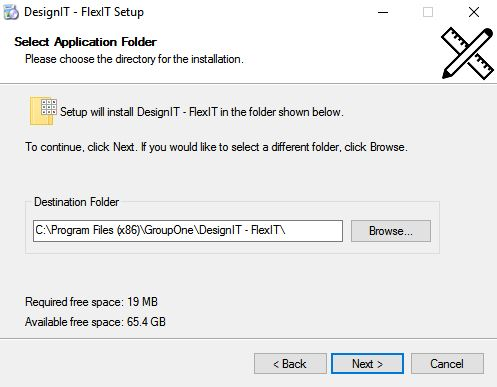
\includegraphics[width=13cm]{images/setup}
\caption{The installer of the software}
\centering
\end{figure}

\section{Code refactoring}

The major problem we had with the source code was inconsistency. Throughout the code we saw different coding styles, lots of redundant codes and unnecessary comments, which made us spend more time on understanding the code base. During this period, we have tried our best to reformat the code. To do so, we were following the conventions described in Google's C++ style guide [6]. 

The first step was to reorganize the projects. Initially we had 3 separate projects, we moved them under one solution, so they can share settings and dependencies (later we also merged two of these project, namely SurfIT and MoveIT into DesignIT), while also allowing us to access them more conveniently.

After that we spent a few days on looking through the source code, while also making it easier to read and shorter, due to removing redundant code chunks and functions. In overall we have managed to reduce the amount of source code by x \% (from y lines of code to z lines of code), while preserving every functionality and also adding many features and bugfixes.

\todo{add actual numbers}

\section{DesignIT}

\section{GUI improvements}

\section{Bugfixes}

During the development we have fixed numerous bugs in the code, improving the overall user experience by a lot. This is the list of the major bugfixes.

\begin{itemize}
\item Menu icons are not visible in the distributed program
\item The icon of the exe files are not visible
\item Cancelling the 'Save As' operation results in error
\todo{list more bugfixes}
\end{itemize}

%%%%%%%%%%%%%%%%%%%%%%%%%%%%%%%%%%%%%%%%%%%%%%%%%%%%%%%%%%%%%%%%%%%%%%%%%%%%%%%%%%%%%%%%%%%%%%%%%%%%%%%

\chapter{Testing and results}

%%%%%%%%%%%%%%%%%%%%%%%%%%%%%%%%%%%%%%%%%%%%%%%%%%%%%%%%%%%%%%%%%%%%%%%%%%%%%%%%%%%%%%%%%%%%%%%%%%%%%%%

\chapter{Conclusion}

%%%%%%%%%%%%%%%%%%%%%%%%%%%%%%%%%%%%%%%%%%%%%%%%%%%%%%%%%%%%%%%%%%%%%%%%%%%%%%%%%%%%%%%%%%%%%%%%%%%%%%%

\chapter{Appendices}

\section{Source code - GitHub}

We have sent the source code via e-mail to Dr. Moulitsas, but our source code is available on GitHub as well. We had to store it in a private repository for safety reasons and due to this, an e-mail must be sent to the owner of the repository (g.szucs@cranfield.ac.uk) with a valid GitHub username, to get access to it. 

\section{Project task management - Trello}

As we discusses before, we have used Trello throughout the whole project to manage our work. It is also a private storage, hence the same routine is needed as for GitHub. Please kindly send a valid Trello username to the same e-mail address to be granted access to our project table. 

%%%%%%%%%%%%%%%%%%%%%%%%%%%%%%%%%%%%%%%%%%%%%%%%%%%%%%%%%%%%%%%%%%%%%%%%%%%%%%%%%%%%%%%%%%%%%%%%%%%%%%%

\begingroup
\renewcommand{\section}[2]{}%
\begin{thebibliography}{1}

\bibitem{c1} J. Katz, A. Plotkin, “Low-speed Aerodynamics”, Cambridge University Press, 2001.

\bibitem{c2} R. Palacios, J. Murua, R. Cook “Structural and Aerodynamic Models in Nonlinear Flight Dynamics of Very Flexible Aircraft”, AIAA Journal 48:2648-2659, 2010.

\bibitem{c3} J. Murua, R. Palacios, J. Michael, R. Graham, “Applications of the Unsteady Vortex-Lattice Method in Aircraft Aeroelasticity and Flight Dynamics”, Department of Aeronautics, Imperial College, London SW7 2AZ, 2012.

\bibitem{c4} S. Cook, “CUDA Programming: A Developer's Guide to Parallel Computing with GPUs (Applications of Gpu Computing)”, Morgan Kaufmann 1st Edition, 2012

\bibitem{c5} J. Cheng, M. Grossman, T. McKercher, “Professional CUDA C Programming”, Wrox 1st Edition, 2014

\bibitem{c6} Google C++ Style guide available at https://google.github.io/styleguide/cppguide.html, 02/05/2017

\end{thebibliography}
\endgroup
   
\end{document}